%% Elsevier article, converted from the Springer LNCS manuscript.
%% Class options: preprint = single column, the layout Elsevier expects for
%% submission.  Swap for [final,5p,times,twocolumn] to preview the journal layout.
\documentclass[final,5p,times,twocolumn,a4paper]{elsarticle}

%% --- Encoding & fonts
\usepackage[T1]{fontenc}
\usepackage[utf8]{inputenc}

%% --- Math
\usepackage{amsmath,amssymb}

%% --- Tables & figures
\usepackage{graphicx}
\usepackage{array}
\usepackage{booktabs}
\usepackage{multirow}
\usepackage{longtable}
\usepackage{float}
\usepackage{tikz}
\usetikzlibrary{positioning,fit,backgrounds,arrows.meta}

%% --- Lists
\usepackage{enumitem}

%% --- Code listings (Python)
\usepackage{xcolor}
\usepackage{listings}
\definecolor{codeblue}{RGB}{0,102,204}
\definecolor{codegray}{RGB}{128,128,128}
\definecolor{codegreen}{RGB}{0,128,0}
\definecolor{backcolour}{RGB}{248,248,248}
\lstdefinestyle{pythonstyle}{
  backgroundcolor=\color{backcolour},
  commentstyle=\color{codegreen}\itshape,
  keywordstyle=\color{codeblue}\bfseries,
  stringstyle=\color{red},
  basicstyle=\ttfamily\small,
  frame=single,
  rulecolor=\color{black},
  numbers=left,
  numberstyle=\tiny\color{codegray},
  breaklines=true,
  breakatwhitespace=true,
  showstringspaces=false,
  tabsize=2,
  captionpos=b
}
\lstset{style=pythonstyle, language=Python}

%% --- URLs & links (hyperref last)
\usepackage[hyphens]{url}
\Urlmuskip=0mu plus 1mu\relax
\usepackage[hidelinks]{hyperref}

%% Long \texttt{} identifiers and URLs cannot be hyphenated; let TeX stretch
%% the interword space a little rather than run into the margin.
\emergencystretch=3em

%% Float placement: this paper has ten full-width tables. The defaults allow
%% only two double-column floats per page, so they accumulate and push the
%% closing sections apart. These values let them settle near their text.
\setcounter{topnumber}{4}
\setcounter{dbltopnumber}{4}
\setcounter{totalnumber}{6}
\renewcommand{\topfraction}{0.92}
\renewcommand{\dbltopfraction}{0.92}
\renewcommand{\bottomfraction}{0.60}
\renewcommand{\textfraction}{0.06}
\renewcommand{\floatpagefraction}{0.75}
\renewcommand{\dblfloatpagefraction}{0.75}

\begin{document}

\begin{frontmatter}

\title{Bringing SQL Row Pattern Matching \texttt{MATCH\_RECOGNIZE} Operator to
  Pandas DataFrames}

%% ORCID iDs from the LNCS version:
%%   Monier Lawande 0009-0002-6531-8709, Ahmed Awad 0000-0003-1879-1026
\author[nu]{Monier Lawande}
\ead{m.ashraf2288@nu.edu.eg}

\author[nu]{Mohamed Elhelw}
\ead{melhelw@nu.edu.eg}

\author[buid,cu]{Ahmed Awad}
\ead{ahmed.awad@buid.ac.ae}

\affiliation[nu]{organization={Center for Informatics Science (CIS), School of
    Information Technology and Computer Science (ITCS), Nile University},
  city={Giza},
  country={Egypt}}

\affiliation[buid]{organization={British University in Dubai},
  city={Dubai},
  country={UAE}}

\affiliation[cu]{organization={Cairo University},
  city={Giza},
  country={Egypt}}

\begin{abstract}
The SQL standard introduced the \texttt{MATCH\_RECOGNIZE} operator in 2016 to support row pattern recognition, enabling the detection of ordered sequences of rows in a table that match a user-defined pattern. This capability is useful in diverse domains—for example, a financial institution may detect a sequence of small deposits followed by rapid transfers and large withdrawals, a known indicator of potential money laundering, or climate analysts may identify heatwaves as three or more consecutive days with maximum temperatures exceeding 40°C.
\texttt{MATCH\_RECOGNIZE} is now supported by several leading database systems, such as Oracle, Snowflake, and Flink. In this paper, we present a prototype that brings this functionality to Pandas DataFrames, a widely used in-memory data structure in the Python data science ecosystem. Our prototype parses SQL-based pattern queries that execute
\texttt{MATCH\_RECOGNIZE()} queries directly from an SQL string on a \texttt{pandas} DataFrame. The system supports SQL:2016 row pattern recognition (RPR) semantics, including \texttt{PARTITION BY}, \texttt{ORDER BY}, \texttt{PATTERN}, \texttt{DEFINE}, and \texttt{MEASURES} for offline analytics in Python. constructs an abstract syntax tree (AST), translates patterns into non-deterministic finite automata (NFA), and executes them efficiently over DataFrames. We evaluate the engine against Trino~473 and Oracle~21c EE on the Amazon UK
Products dataset, running five pattern families over six sizes up to 2,222,742
rows. The three systems return identical results in all 30 pattern--size cells,
and the engine averages 0.17 seconds per cell against 1.04 for Oracle and 1.98
for Trino. A scalability test on the Amazon Reviews 2023 corpus extends the
input to 227,899,533 rows, which the engine completes on every pattern family.
The declarative form also reduces code size compared to native Pandas
implementations, extending the convenience of SQL pattern matching to Python
users while preserving correctness equivalent to that of established SQL
engines.
\end{abstract}

\begin{keyword}
Pattern Matching \sep MATCH\_RECOGNIZE \sep Pandas \sep SQL \sep Finite Automata \sep Data Engineering
\end{keyword}

\end{frontmatter}

\section{Introduction}
Pattern matching is the process of analyzing a sequence of data points, which can be rows in a table or events in a stream. Pattern matching plays a crucial role in data analysis, especially for identifying patterns and shapes or specific sequences of events or behaviors in areas like identifying chains of transactions related to money laundering in finance\cite{10.5120/ijca2022922446}, revealing fraudulent behaviours of users in security logs\cite{zemke2007pattern}. Patterns in data can be described using regular-expression-like syntax, like those commonly used in textual analysis. However, unlike traditional text-based regular expressions, these patterns are applied at the row level, enabling analysts to match and extract meaningful sequences across entire records rather than individual characters.

The \texttt{MATCH\_RECOGNIZE} (MR) clause was introduced in the SQL:2016 standard \cite{iso2016,ISO2021}, enabling users to define and search for patterns within ordered sequences of rows directly in SQL queries.
The {MATCH\_RECOGNIZE} SQL clause enables advanced pattern-based querying over data tables. Although it was standardized in SQL:2016 \cite{iso2016,ISO2021}, a few DBMS support it. For example, among well-known traditional RDBMSs, only Oracle\cite{oracle2022,book} supports the MR operator. In the big data analytics systems, Trino~\cite {trino2022,trino2021row}, Snowflake~\cite{snowflake2025match_recognize}, and Apache Flink~\cite{flink} support the MR operator.
Cloud warehouses have since followed: BigQuery documents the
clause~\cite{bigquery2025matchrecognize}, and Databricks introduced beta
support in Runtime~19.0~\cite{databricks2026matchrecognize}. By contrast,
PostgreSQL~18 still lists the related SQL features as
unsupported~\cite{postgresql18unsupported}, while DuckDB lists native
\texttt{MATCH\_RECOGNIZE} as planned work~\cite{duckdb2026roadmap}. 

% and it was supported in several modern databases like Trino  and Oracle , this feature is missing from the Python data science landscape. In this paper, we address this gap by bringing \texttt{MATCH\_RECOGNIZE} support to Pandas.

Without the support for the declarative MR clause, tasks requiring detecting multi-row patterns often require complicated combinations of SQL window functions, self-joins, or even procedural extensions and user-defined functions to loop through rows and maybe add some external programming outside the database~\cite{findling2025bringing}. As soon as the pattern grew beyond two or three steps, the SQL statement expanded into multiple lines full of row-number calculations, timestamp comparisons, and complex JOIN conditions. Not only is the code hard to write and even harder to maintain, but each extra join or analytic window often means an extra table scan, leading to poor performance. In practice, many teams either accepted these limitations or abandoned SQL for external scripts and ETL pipelines just to get reliable pattern matching SQL expanded into multiple lines~\cite{cao2012optimizationanalyticwindowfunctions}.

With the introduction of MATCH\_RECOGNIZE in the SQL:2016 standard, rather than a multitude of lines of code and using window functions and self-joins, Instead, a single declarative MATCH\_RECOGNIZE statement that clearly defines the data partitions, ordering, pattern, and output measures. Simplifying both the syntax and readability of pattern-matching queries, MATCH\_RECOGNIZE clause enables users to organize their data into logical groups using \texttt{PARTITION BY}, specify the sequence of row analysis using  \texttt{ORDER BY}, and define the actual pattern using the \texttt{PATTERN} section, which uses regular expression-like syntax. Logical conditions that define each pattern element are clearly stated in the \texttt{DEFINE} clause, while the \texttt{MEASURES} clause determines what information is extracted from each detected match. This structure allows complex sequence patterns to be described clearly and concisely. It ensures that detecting, classifying, and summarizing sequences can be performed efficiently and consistently within standard SQL queries, such as trends, repeated behaviors, or sudden changes, directly within standard SQL queries \cite{michels2018new}.

%the following has nothing new complexity-wise. It does not matter if this is Pandas or any other other DBMS that provides its own programming language.

% we need instead to motivate that PANDAS is a powerful libarary for (multi-dimensional ) tabular data processing for several data analytics projects. Despite its powwer, it provides its own DSL (imperative language) to compute data transformations. 

% The contribution, in this paper, we bring the power of row pattern matching using Match_recognize on top of PANDAS. this should boost the performance of data analysts and ML engineerings by declaratively and succinctly defining their patterns and using the reulsts for further analysis of engineering features for their ML models.

Before introducing the MATCH\_RECOGNIZE method in Pandas, detecting multi-row patterns such as consecutive upward trends, cyclical oscillations, or conditional event sequences required manual integration of multiple low-level operations. A typical workflow involved creating multiple shifted versions of each column (df['value'].shift(-1), shift(-2), etc.), building complex boolean masks, filtering or using groupby().apply() to stitch subsequences back together, and then pivoting or renaming columns to get the desired output. This approach was verbose (often 10+ lines for modest patterns), prone to off-by-one or alignment bugs, and hard to extend to longer or conditional patterns.

For example, an e-commerce platform that tracks all customer purchases: the marketing team wants to find customers who are decreasing their spending money by buying progressively cheaper items in three consecutive purchases, by detecting three consecutive purchases using pandas functions for pattern (A B C).
\begin{lstlisting}[basicstyle=\ttfamily\footnotesize,language=Python,
                   caption={Apply \texttt{MATCH\_RECOGNIZE} using pandas functions},
                   label={lst:UDF-match-recognize},
                   frame=single]
import pandas as pd
df['order_date'] = pd.to_datetime(df['order_date'])
# Sort for partition
df = df.sort_values(['customer_id', 'order_date']).reset_index(drop=True)
def match_pattern_ABC(group: pd.DataFrame):
    """Find matches where B.price < A.price and C.price < B.price."""
    matches = []
    n = len(group)
    for i in range(n - 2):  # need at least 3 rows for A,B,C
        A = group.iloc[i]
        B = group.iloc[i + 1]
        C = group.iloc[i + 2]

        if (B['price'] < A['price']) and (C['price'] < B['price']):
            matches.append({
                'customer_id': A['customer_id'],
                'start_date': A['order_date'],
                'end_date': C['order_date'],
                'bottom_price': C['price']
            })
    return matches
# Apply per partition
all_matches = []
for cust_id, grp in df.groupby('customer_id'):
    all_matches.extend(match_pattern_ABC(grp))

result_df = pd.DataFrame(all_matches)
print(result_df)
\end{lstlisting}




After integrating MATCH\_RECOGNIZE into Pandas, the complex operations that were applied before were eliminated. In a single statement, it is possible to define partitioning column(s), ordering key, pattern grammar (e.g., "A B C"), logical definitions for each step, and the summary or detail measures that will be returned. The method returns a clean, annotated DataFrame of full matches. Additionally, it is simple to expand to more intricate patterns, varying lengths, or conditional patterns; simply update the pattern string or definitions to align with specifications. Using the same declarative SQL syntax can be effectively utilized for multiple analytical use cases \cite{petkovic2022rpr}.

\noindent\textbf{The MATCH\_RECOGNIZE clause:}
\begin{lstlisting}[language=SQL,frame=single]
SELECT <columns to return>
FROM <table_name>
MATCH_RECOGNIZE
(
  [ PARTITION BY <columns to group data by> ]
  [ ORDER BY <columns to sort each group> ]
  [ MEASURES <expressions to define output values> ]
  [ ONE ROW PER MATCH | ALL ROWS PER MATCH ]
  [ AFTER MATCH <skip to option> ]
  [ PATTERN ( pattern_expression ) ]
  [ SUBSET <combine multiple variables into one> ]
  DEFINE <rules for each pattern variable>
);
\end{lstlisting}

\noindent\textbf{Core Components of Row Pattern Recognition:}

Row pattern recognition in SQL, as standardized in SQL:2016, detects patterns in sequential data through the 
\texttt{MATCH\_RECOGNIZE} clause. The foundational architecture establishes independent pattern matching scopes via \texttt{PARTITION BY} clauses and defines temporal ordering through \texttt{ORDER BY} specifications within each partition. Pattern definitions utilize regular expression-inspired syntax (e.g., A B+ C?) to express complex event sequences, incorporating fundamental operations such as concatenation, alternation, and quantified repetition through standard quantifiers (\texttt{*}, \texttt{+}, \texttt{?}, \texttt{\{n,m\}}). The \texttt{DEFINE} clause establishes boolean predicates for pattern variables, enabling the incorporation of navigation functions (\texttt{FIRST}, \texttt{LAST}, \texttt{PREV}, \texttt{NEXT}) that facilitate temporal and positional analysis of data relationships with appropriate boundary condition handling. The \texttt{MEASURES} clause enables the extraction of computed values from successful pattern matches, supporting standard functions including \texttt{CLASSIFIER()} for pattern variable identification and \texttt{MATCH\_NUMBER()} for match sequence enumeration, with dual semantic evaluation modes: \texttt{RUNNING} for incremental computation and \texttt{FINAL} for complete match evaluation. \texttt{SUBSET} variables provide pattern abstraction capabilities through hierarchical variable grouping mechanisms.
Pattern anchors (\texttt{\^{}}, \texttt{\$}), exclusion blocks
(\texttt{\{-~\ldots~-\}}), and \texttt{PERMUTE} extend the pattern language
further, and a variable used in \texttt{PATTERN} without a \texttt{DEFINE}
predicate is treated as implicitly true. Match control policies, implemented via \texttt{AFTER MATCH SKIP} directives, govern result cardinality and pattern overlap behavior while determining continuation strategies for subsequent pattern detection iterations, ensuring deterministic matching behavior in compliance with SQL:2016 specifications.
% explicitly mention the contributions

For example, an e-commerce platform that tracks all customer purchases, the marketing team wants to
find customers who are decreasing their spending money by buying progressively cheaper items in three
consecutive purchases, by detecting three consecutive purchases using MATCH\_RECOGNIZE for the pattern (A B C).
\begin{lstlisting}[language=Python,
                   caption={Using \texttt{MATCH\_RECOGNIZE}},
                   label={lst:basic-match-recognize},
                   frame=single]
import pandas as pd
from src.executor.match_recognize import match_recognize
df['order_date'] = pd.to_datetime(df['order_date'])
# Define the MATCH_RECOGNIZE query
query = """
SELECT customer_id, start_date, end_date, bottom_price
FROM orders
MATCH_RECOGNIZE (
  PARTITION BY customer_id
  ORDER BY order_date
  MEASURES
    A.order_date AS start_date,
    C.order_date AS end_date,
    C.price      AS bottom_price
  PATTERN (A B C)
  DEFINE
    B AS B.price < A.price,
    C AS C.price < B.price
);
"""
# Execute and print results
output_df = match_recognize(query, df)
print(output_df)
\end{lstlisting}


\section{Background and Related Work} 
The SQL:2016 \texttt{MATCH\_RECOGNIZE} clause is supported by many leading SQL engines natively, like Oracle\cite{oracle2022,book}, Snowflake\cite{snowflake2025match_recognize}, and Trino \cite {trino2022,trino2021row} and others while still under consideration to implement this feature, like PostgreSQL \cite{howe2020matchrecognize}, MariaDB \cite{mariadb2025regex}, and Microsoft SQL Server \cite{10.14778/3579075.3579090}, To use \texttt{MATCH\_RECOGNIZE} in these systems without native support, users must emulate row-pattern matching using a combination of window functions, user-defined aggregates, or external procedural layers—approaches that are often more complex, less efficient, and harder to maintain, or external processing layers~\cite{TURP2,TURP}.
A different route is translation: the database group at the University of
T\"ubingen rewrites row-pattern queries into recursive common table expressions
that DuckDB already executes~\cite{findling2025bringing}, which avoids adding a
native operator but still requires a second engine. The landscape continues to
move: BigQuery documents the clause~\cite{bigquery2025matchrecognize} and
Databricks offers it in beta~\cite{databricks2026matchrecognize}, while
PostgreSQL~18~\cite{postgresql18unsupported} and
DuckDB~\cite{duckdb2026roadmap} still list it as absent or planned.




\subsection{Pandas}

Pandas is a popular, open-source Python library for data analysis and manipulation. Its straightforward installation process and strong community support make it a good choice for students, researchers, and professionals who frequently need to analyze data without using complicated systems like Oracle, Trino, or Snowflake. For everyday tasks, Pandas offers straightforward methods for managing data sequences, filtering, grouping, and performing basic time-series analyses. However, it has difficulty with advanced pattern detection in contrast to SQL's \texttt{MATCH\_RECOGNIZE} clause. Pandas lacks a straightforward way to express complex patterns, users must create their own solutions using functions like \texttt{rolling}, \texttt{groupby}, or \texttt{shift}. These custom approaches can become complicated and error-prone, especially with advanced patterns. Pandas is highly popular due to ease of setup and use, absence of licensing fees, and smooth integration within the larger Python libraries. This makes it great for quickly developing and testing ideas for typical pattern detection needs.

\subsection{Existing Implementations}

Oracle \cite{oracle2022,book}, Trino \cite {trino2022,trino2021row}, Snowflake \cite{snowflake2025match_recognize}, and Flink \cite{flink} all provide advanced solutions for SQL-based pattern matching, but they each come with important practical challenges that users need to keep in mind. Oracle provides a comprehensive and robust implementation of the \texttt{MATCH\_RECOGNIZE} clause, well-suited for complex, enterprise-scale analytics. However, this power comes with high operational costs (including licensing fees). 
Trino, an open-source alternative, supports \texttt{MATCH\_RECOGNIZE} with a syntax close to the SQL:2016 standard and performs well in distributed data environments. It is more accessible than Oracle in terms of deployment and cost, but still requires considerable infrastructure management and may lack some of Oracle’s advanced optimizations. Snowflake is a cloud-native platform that is scalable and provides a user-friendly MATCH\_RECOGNIZE feature for identifying common event patterns. However, offers limited support for advanced clauses and has computational costs that relate to the size of the warehouse. Apache Flink is designed for real-time stream processing, allowing rapid detection of event patterns in continuous data flows. While Flink is highly scalable and effective for high-velocity data, it introduces its own learning curve and is less familiar to users accustomed to traditional, batch-based SQL systems \cite{vsprem2024building,georgiou2025streaming}.\\

A major limitation shared by all these platforms is the complexity of integrating SQL-based pattern matching with machine learning workflows and other analytics tools~\cite{ML_Workflow,Makrynioti2019sql4mlAD}. Typically, data must be exported from the database to external environments for ML modeling, resulting in data duplication, consistency challenges, and more complicated data pipelines \cite{naphade2025evolution}. Keeping track of multiple versions of the same dataset across systems also increases the risk of errors and inefficiency. For many users especially those with modest analytics needs or who work independently, installing and managing large-scale systems like Oracle, Trino, Snowflake, or Flink can be overly complicated for some users. These users may only need to perform occasional pattern detection and would prefer to avoid the overhead of learning different functions or dealing with varying syntax for similar queries across platforms \cite{8509400}. Additionally, for datasets that fit comfortably in memory, tools like Pandas offer a faster and more direct alternative, eliminating the latency of disk-based operations common to larger database engines\cite{Evaluation,in-memory_processing}.
Although Oracle, Trino, Snowflake, and Flink each have unique strengths for SQL pattern matching in large-scale or real-time scenarios, they introduce extra costs, infrastructure requirements, and integration issues that can be prohibitive for everyday users. These limitations highlight the value of Pandas, as it offers simpler, memory-based tools and unified workflows, where pattern matching and data analytics can be performed seamlessly and without unnecessary duplication or complexity.

\section{System Design and Methodology}

Our \texttt{MATCH\_RECOGNIZE} implementation follows a modular, five-stage architecture specifically designed for SQL row pattern recognition. The engine executes SQL queries directly on \texttt{pandas} DataFrames~\cite{monierashraf2025rowmatch}, while fully preserving SQL:2016 semantics~\cite{iso2016,ISO2021,melton2017sqlrpr}. The pipeline consists of five phases: parsing, semantic validation, logical plan construction, pattern compilation, and execution (Fig.~\ref{fig:system-architecture}).

In the parsing stage, the SQL query is transformed into an abstract syntax tree (AST) that captures both the \texttt{SELECT}/\texttt{FROM} clauses and \texttt{MATCH\_RECOGNIZE} subclauses~\cite{tarazona2021antlr,parr2013definitive}. Semantic validation then checks schema references, variable usage, predicates, skip policies, and output modes. Compliance rules are applied to ensure standard conformance, correct use of navigation functions, consistent measure semantics, and robust handling of edge cases such as empty matches, partition boundaries, and skip behaviors.

The validated plan is translated into a logical plan composed of modular operators for partitioning, sorting, matching, measuring, and skipping. From this plan, the system compiles a nondeterministic finite automaton (NFA) with guarded transitions that support quantifiers, alternation, and
\texttt{PERMUTE} constructs~\cite{salomaa1996nfa}. The NFA is constructed using Thompson’s construction, extended for
SQL:2016 semantics by embedding predicates from the \texttt{DEFINE} clause, minimizing epsilon transitions, and applying subset construction with state deduplication to mitigate exponential growth.
Because subset construction is exponential in the worst case, the compiler is
guarded: \texttt{PERMUTE} is rejected above eight variables or an estimated
50,000 branches, and DFA construction stops at a ceiling of 50,000 states.
Exceeding any guard raises an explicit compilation error, so the engine never
executes or caches a partial automaton.

Finally, execution is performed over ordered partitions using the compiled automaton. Matches are materialized with the correct \texttt{RUNNING}/\texttt{FINAL} semantics. The evaluation engine manages context separation, applies navigation functions (\texttt{FIRST}, \texttt{LAST}, \texttt{PREV}, \texttt{NEXT}) with partition awareness, and computes aggregates such as \texttt{COUNT}, \texttt{SUM}, and \texttt{AVG} across pattern variables. This ensures full compliance with SQL:2016 while producing results directly as \texttt{pandas} DataFrames.




\begin{figure}[t]
\centering
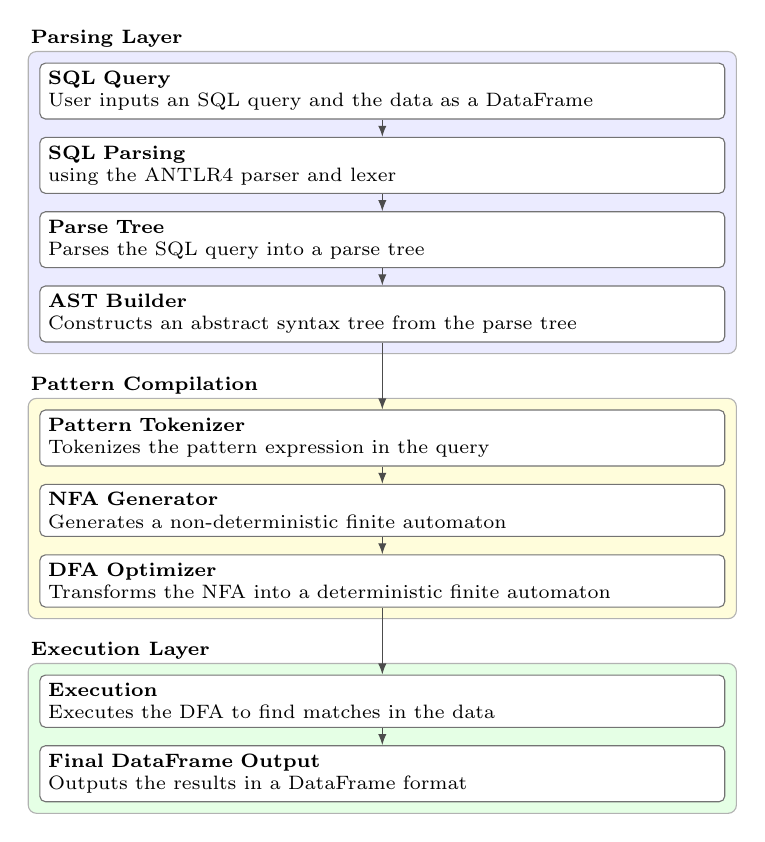
\begin{tikzpicture}[
  font=\scriptsize,
  box/.style={draw=black!55, rounded corners=2pt, fill=white, align=left,
              text width=0.70\columnwidth, inner sep=3pt},
  band/.style={rounded corners=3pt, draw=black!30, inner sep=4pt},
  lbl/.style={font=\scriptsize\bfseries, inner sep=1pt},
  arr/.style={-{Latex[length=4pt,width=3pt]}, draw=black!70}]

  \node[box] (q)  {\textbf{SQL Query}\\User inputs an SQL query and the data as a DataFrame};
  \node[box, below=2.2mm of q]  (sp) {\textbf{SQL Parsing}\\using the ANTLR4 parser and lexer};
  \node[box, below=2.2mm of sp] (pt) {\textbf{Parse Tree}\\Parses the SQL query into a parse tree};
  \node[box, below=2.2mm of pt] (ab) {\textbf{AST Builder}\\Constructs an abstract syntax tree from the parse tree};

  \node[box, below=8.5mm of ab]   (tk) {\textbf{Pattern Tokenizer}\\Tokenizes the pattern expression in the query};
  \node[box, below=2.2mm of tk] (nf) {\textbf{NFA Generator}\\Generates a non-deterministic finite automaton};
  \node[box, below=2.2mm of nf] (df) {\textbf{DFA Optimizer}\\Transforms the NFA into a deterministic finite automaton};

  \node[box, below=8.5mm of df]   (ex) {\textbf{Execution}\\Executes the DFA to find matches in the data};
  \node[box, below=2.2mm of ex] (out){\textbf{Final DataFrame Output}\\Outputs the results in a DataFrame format};

  \foreach \a/\b in {q/sp, sp/pt, pt/ab, ab/tk, tk/nf, nf/df, df/ex, ex/out}
    \draw[arr] (\a) -- (\b);

  \begin{scope}[on background layer]
    \node[band, fill=blue!8,   fit=(q)(ab),  label={[lbl,anchor=south west]north west:Parsing Layer}]      {};
    \node[band, fill=yellow!14, fit=(tk)(df), label={[lbl,anchor=south west]north west:Pattern Compilation}]{};
    \node[band, fill=green!10,  fit=(ex)(out),label={[lbl,anchor=south west]north west:Execution Layer}]    {};
  \end{scope}
\end{tikzpicture}
\caption{System architecture.}
\label{fig:system-architecture}
\end{figure}


\subsection{SQL Parsing and AST Construction}


The process starts by analyzing the user's SQL query, identifying its logical components. This proceeds through a parsing process that explores the query, recognizes its main components such as grouping (\texttt{PARTITION BY}), ordering (\texttt{ORDER BY}), the pattern to be searched, and any specific conditions or output metrics, and then organizes these into an Abstract Syntax Tree (AST). The AST provides a clear and structured representation of the query. This approach eases query validation and prepares it for pattern matching in the following stages.


\subsection{Pattern Translation to Finite Automata}

Once the AST is completed, the system focuses on the pattern component described in the SQL query. This pattern is then converted into a finite automaton, which defines a set of states and transitions for detecting complex sequences or behaviors in the data. 
This process begins by constructing a non-deterministic finite automaton (NFA) from the pattern and then, for improved efficiency, transforms it into a deterministic finite automaton (DFA) \cite{georgiou2025streaming}. The DFA  enhances the matching process by removing ambiguity in transitions, enabling the system to scan data sequences quickly and accurately. This translation process enables the system to handle a wide variety of pattern features, such as repetitions, alternatives, and specific sequences, in a unified and efficient way. The resulting automaton acts as the core mechanism for scanning and detecting patterns within the data.


\subsection{Execution Engine on Pandas}

The execution phase uses the constructed DFA to perform pattern matching directly over input data represented as Pandas DataFrames. The engine begins by partitioning and ordering the data according to the query’s specifications. It then applies the DFA to scan the dataset, identifying all sequences that fit the defined pattern. For every detected match, the engine computes any requested measures or calculations and compiles the results into a DataFrame formatted to mirror standard SQL query outputs. By utilizing Pandas, the system retains both flexibility and accessibility, smoothly incorporating advanced pattern matching into conventional Python data analysis workflows.

\section{Implementation and Optimization}

\subsection{ANTLR4 Grammar and AST Construction}
 Our system uses a customized SQL grammar, extended from Trino’s SQL that fully supports the SQL:2016 \texttt{MATCH\_RECOGNIZE} clause. This grammar was defined by ANTLR4, including complex patterns, nested patterns, alternation, quantifiers, grouping, and exclusions \cite{antlr_trino_sql}. The parser’s output is a detailed parse tree that captures the syntactic structure of each SQL query\cite{parr2013definitive},\cite{tarazona2021antlr}.
 
\subsection {Finite Automata }
{Pattern Tokenization,}
Pattern expressions are tokenized using a recursive descent tokenization algorithm that supports anchors, grouping, quantifiers, and nested constructs.

{NFA Construction,}
We use Thompson’s construction algorithm to translate pattern tokens into a Non-deterministic Finite Automaton (NFA). Each state captures transitions, variable bindings, anchors, and metadata for advanced features. Quantifiers (\texttt{*}, \texttt{+}, \texttt{?}, \texttt{\{n,m\}}) are directly mapped to sub-automata \cite{georgiou2025streaming}.

{DFA Construction and Optimization,}
The NFA is systematically converted into a Deterministic Finite Automaton (DFA) using subset construction, drastically reducing the number of active states during execution. Using optimization steps like state minimization, transition indexing, and merging equivalent states results in a compact and performant automaton. The resulting DFA supports efficient row-by-row evaluation while preserving pattern semantics and priorities and custom conditions for accurate pattern semantics \cite{e104-d_3_381,10.1145/986537.986588,georgiou2025streaming}.

\subsection {Execution}

The matching engine applies the DFA sequentially over each partition of the DataFrame with specialized handling for anchors, skip modes, and edge cases. The executor coordinates the entire pattern matching process, integrating parsing, automata construction, match identification, and result formatting.

{Condition and Measure Evaluation,}
A dedicated evaluation subsystem translates SQL pattern conditions and measures into executable Python code  that supports navigation functions and aggregations with SQL:2016 compliant NULL semantics for both running and final calculations.\\

\section{Experimental Evaluation}

\subsection{Evaluation Methodology}

\subsubsection{Evaluation Criteria and Metrics}

We evaluate the proposed \texttt{MATCH\_RECOGNIZE} engine through five criteria.
First, \texttt{output correctness}: results are compared with Trino 473 and
Oracle 21c EE by row-level equality across multiple pattern types, ensuring
identical matching, pattern alignment, and measure calculations. Second,
\texttt{semantic coverage}: following SQL:2016 \texttt{MATCH\_RECOGNIZE}
semantics—including \texttt{PERMUTE} patterns, exclusions, quantifiers,
navigation functions, and output modes—and compatibility with standard SQL
semantics \cite{iso2016,ISO2021,monierashraf2025rowmatch}. Third,
\texttt{developer effort (code size)}: the lines required to express equivalent
logic in idiomatic \texttt{pandas}; baselines typically need substantially more
code (e.g., chained \texttt{groupby}/\texttt{shift}/joins) than a single
\texttt{MATCH\_RECOGNIZE} statement, yielding reduced LOC in line with the row
pattern recognition (RPR) goal of lowering implementation effort
\cite{iso2016,ISO2021,melton2017sqlrpr,Python_UDF}. Fourth,
\texttt{performance}: client-observed execution time, throughput, and memory
for every pattern--size cell, where each cell is the mean of twenty measured
runs after five warm-up runs and outliers are removed by the 1.5$\times$
interquartile range rule. Fifth, \texttt{scalability}: how execution time and
memory grow as the input grows, measured on real data up to 227,899,533 rows.




\subsubsection{Environment and Configuration}

The experiments were performed on a workstation running Ubuntu 24.04.4 LTS with an Intel Core i7\-11800H (16 cores at 2.30 GHz) and 64 GB of DDR4 RAM at 3200 MHz. The software setup uses Trino 473 (baseline SQL engine); Java 11.0.25 LTS and Python 3.12.7; Python libraries including \texttt{pandas} 2.3.3, \texttt{numpy} 2.1.3, \texttt{antlr4-python3-runtime} 4.13.2, \texttt{antlr4-tools} 0.2.1, \texttt{pytest} 8.3.4, Jupyter, \texttt{unittest}, \texttt{matplotlib} 3.10.0, \texttt{plotly} 5.24.1, and \texttt{seaborn} 0.13.2; and standard libraries such as \texttt{typing}, \texttt{dataclasses}, \texttt{re}, \texttt{operator}, \texttt{math}, \texttt{itertools}, \texttt{collections}, \texttt{enum}, \texttt{time}, \texttt{sys}, \texttt{os}, \texttt{logging}, and \texttt{traceback}. 
\texttt{MATCH\_RECOGNIZE} implementation using ANTLR4 for parsing Trino SQL, \texttt{pandas} for DataFrame management, and custom AST/NFA/DFA modules for pattern detection.





\subsection{Dataset and Test Patterns}

We use an Orders table to demonstrate and validate pattern-matching queries. The dataset comprises three attributes\cite{trino2021row}:

\texttt{customer\_id} (VARCHAR), which identifies the customer (two distinct values: \texttt{cust\_1} and \texttt{cust\_2}); \texttt{order\_date} (DATE), the date the order was placed (ranging from May~11,~2020 to May~18,~2020); and \texttt{price} (INTEGER), the purchase amount on that date. Table~\ref{tab:orders} shows a sample of data from eight records:


\begin{table*}[t]
  \centering\small
  \caption{Sample “orders” dataset (\texttt{customer\_id}, \texttt{order\_date}, \texttt{price})}
  \label{tab:orders}
  \begin{tabular}{lcr}
    \toprule
    \textbf{customer\_id} & \textbf{order\_date} & \textbf{price} \\
    \midrule
    cust\_1 & 2020-05-11 & 100 \\
    cust\_1 & 2020-05-12 & 200 \\
    cust\_2 & 2020-05-13 &   8 \\
    cust\_1 & 2020-05-14 & 100 \\
    cust\_2 & 2020-05-15 &   4 \\
    cust\_1 & 2020-05-16 &  50 \\
    cust\_1 & 2020-05-17 & 100 \\
    cust\_2 & 2020-05-18 &   6 \\
    \bottomrule
  \end{tabular}
\end{table*}

Since each customer appears multiple times in chronological order with \texttt{cust\_1} spanning five dates and \texttt{cust\_2} spanning three, this table allows us to test pattern‐matching queries (e.g., sequences of rising/falling prices per customer). This dataset structure enables comprehensive validation of partitioning, ordering, and pattern detection. In our experiments, we load this data via a simple SQL VALUES clause and verify that our \texttt{MATCH\_RECOGNIZE} implementation produces exactly the same matched rows and measures as Trino’s \texttt{MATCH\_RECOGNIZE}.\\

\begin{lstlisting}[basicstyle=\ttfamily\small, backgroundcolor=\color{gray!10} ,caption={Creating the in-memory table in Trino }]
CREATE TABLE memory.default.orders (
    customer_id VARCHAR,
    order_date DATE,
    price INTEGER
);

\end{lstlisting}


\begin{lstlisting}[basicstyle=\ttfamily\small, backgroundcolor=\color{gray!10},caption={Inserting data into the table }]

INSERT INTO memory.default.orders
VALUES 
    ('cust_1', DATE '2020-05-11', 100),
    ('cust_1', DATE '2020-05-12', 200),
    ('cust_2', DATE '2020-05-13',   8),
    ('cust_1', DATE '2020-05-14', 100),
    ('cust_2', DATE '2020-05-15',   4),
    ('cust_1', DATE '2020-05-16',  50),
    ('cust_1', DATE '2020-05-17', 100),
    ('cust_2', DATE '2020-05-18',   6);

\end{lstlisting}



\paragraph{Amazon UK Products.}
The performance benchmark uses the Amazon UK Products
dataset~\cite{asaniczka2023amazon}, roughly 2.2\,million product records from
Amazon's UK marketplace in a single CSV file. Four columns are used:
\texttt{stars}, \texttt{reviews}, \texttt{price} (GBP), and
\texttt{categoryName}. A derived \texttt{category} column maps the price into
five bands: A (${\le}$\pounds10), B (\pounds10--25), C (\pounds25--50),
D (\pounds50--100), and E (${>}$\pounds100). Each row carries a sequential
\texttt{seq\_id} in source order.

\paragraph{Amazon Reviews 2023.}
The scalability test needs far more rows than the product table provides, so it
uses the Amazon Reviews 2023 corpus~\cite{hou2024amazonreviews} from the
McAuley Lab at UC San Diego, roughly 571\,million genuine review events. Only
the pattern-relevant fields are taken: \texttt{user\_id},
\texttt{parent\_asin}, \texttt{rating}, and \texttt{timestamp}; review text,
images, and product metadata are excluded. Five categories are merged in global
timestamp order, and each review's 1--5 rating is mapped to the same A--E
alphabet, so the same pattern families apply to both datasets.

\paragraph{Test patterns.}


{\small
\setlength{\LTleft}{0pt}
\setlength{\LTright}{0pt}
\begin{table*}[t]
\centering
\caption{SQL Pattern Definitions and Detection Goals}
\label{tab:pattern_definitions}
\begin{tabular}{@{\extracolsep{\fill}}llp{0.45\textwidth}}
\toprule
\textbf{Pattern Name} & \textbf{SQL Pattern} & \textbf{Description \& Goal} \\
\midrule


simple\_sequence & \texttt{A+ B+} &
\textbf{Goal:} Detect transitions from budget to low-mid price listings. \newline
\textbf{Use:} Identify runs where budget products (${\le}$\pounds10) are immediately followed by low-mid products (\pounds10--25), useful for detecting problematic product sequences or data quality issues in listings. \\
\midrule

alternation & \texttt{A (B|C)+ D} &
\textbf{Goal:} Detect budget-to-upper-mid transitions through mixed middle bands. \newline
\textbf{Use:} Find sequences that start with a budget product, continue with a mix of low-mid and mid products (\pounds10--50), and end with an upper-mid product (\pounds50--100). Useful for analyzing quality improvement patterns in product browsing sequences or sorted lists. \\
\midrule

quantified & \texttt{A\{1,5\} B* C+} &
\textbf{Goal:} Detect bounded budget runs followed by mid-band products. \newline
\textbf{Use:} Find sequences with 1--5 budget products, optionally followed by low-mid products, then one or more mid products (\pounds25--50). Enforces minimum unrated product counts for identifying problematic product clusters. \\
\midrule

optional\_pattern & \texttt{A+ B? C*} &
\textbf{Goal:} Flexible budget-run detection with optional band transitions. \newline
\textbf{Use:} Broad matching of budget runs with an optional low-mid product and optional mid products. High recall for various low-quality sequence scenarios in e-commerce data. \\
\midrule

complex\_nested & \texttt{(A|B)+ (C\{1,3\} D*)+} &
\textbf{Goal:} Nested grouping of low-price runs followed by mid/upper-mid groups. \newline
\textbf{Use:} Detect runs of low-priced products (${\le}$\pounds25) followed by one or more groups of 1--3 mid products with optional upper-mid products. Useful for multi-level quality grouping and advanced sorting pattern detection in product listings. \\
\bottomrule
\end{tabular}
\end{table*}
}

All patterns run on the derived \texttt{category} column, where A is budget (${\le}$\pounds10), B low-mid (\pounds10--25), C mid (\pounds25--50), D upper-mid (\pounds50--100), and E premium (${>}$\pounds100). On the Amazon Reviews corpus the same A--E alphabet is derived from the 1--5 rating.
Table~\ref{tab:pattern_definitions} provides detailed specifications of all five SQL patterns used in the evaluation, including their formal syntax and intended detection goals. Each pattern represents a different complexity level and use case, ranging from simple sequential matching to complex nested structures with quantifiers and alternation operators.





\subsection{Complexity Analysis}

Costs are stated in asymptotic notation over five symbols: $n$ input rows, $m$
pattern symbols, $d$ \texttt{DEFINE} variables, $k$ matches, and $\ell$ the
average number of rows per match materialised in the output, so $\ell = 1$
under \texttt{ONE ROW PER MATCH}. Running a query does five kinds of work:
parsing, automaton construction, ordering, condition checking, and matching
with output construction.

Parsing and automaton construction depend on the pattern rather than on the
data. NFA construction is $O(m)$, and the NFA-to-DFA conversion is $O(2^{m})$
states in the worst case but a handful in practice; for a fixed pattern this is
a one-time constant, and the compiled automaton is cached across queries.
Ordering is the only data-dependent cost above linear: a comparison sort costs
$O(n \log n)$ per partition, but the engine first checks in $O(n)$ whether the
rows already follow the requested order and skips the sort when they do.
Condition checking prepares one Boolean result per row and variable on the
compiled row-local path, costing $O(nd)$, and matching with output construction
then costs $O(n + k\ell)$ on the default-skip path.

Two independent axes follow. Along the data axis, with the pattern fixed, the
engine is $\Theta(nd + n + k\ell) = \Theta(n)$ when the input is already
ordered, as it is in the benchmark, and $O(n \log n)$ when a sort is required,
because $d$ is a property of the query rather than of the table and
$k\ell = O(n)$ while matches do not overlap. Along the pattern axis, with the
data fixed, three constructs are expensive in $m$ rather than in $n$: the
NFA-to-DFA conversion, \texttt{PERMUTE}, which expands to $O(m!)$ branches, and
a \texttt{DEFINE} predicate that reads the match built so far, which cannot use
the row-local Boolean matrix and may require the preference-ordered exact
search. Each of the three is either paid once or held in check by the explicit
compiler guards, so none of them appears as a growth curve in the data size.
The measured times reported below follow the ordered case.

\subsection{Empirical and Cross-System Analysis}\label{sec:empirical}

\subsubsection{Performance results using real dataset}

Two campaigns are run, one on each real dataset. The first measures performance
on the Amazon UK Products data over six nested prefixes: 100K, 200K, 400K,
800K, 1.6M, and the full 2,222,742 rows. The five pattern families of
Table~\ref{tab:pattern_definitions} run at every size, giving 30 pattern--size
cells per system, and Trino 473 and Oracle 21c EE execute the same query bodies
as references. Each cell is the mean of twenty measured runs after five warm-up
runs, with outliers removed by the 1.5$\times$ interquartile range rule. All 90
cells completed, and the three systems returned the same normalised result set
in every cell.

The second campaign tests scalability on the Amazon Reviews corpus over seven
prefixes: 5M, 10M, 20M, 40M, 80M, 160M, and 227,899,533 rows, under a 58\,GB
limit and a 600-second per-query budget, with two warm-up runs and five
measured runs per cell. The same five families are used; four keep the
benchmark structure with rating labels, and the optional family uses
\texttt{E D? C+ B*}. No query uses \texttt{PARTITION BY}, so every run scans a
single partition in order, which removes the parallel work that partitioning
would otherwise allow.


Table~\ref{tab:pattern_summary} summarises each family averaged over the six
sizes. Pattern structure, not match volume, drives the cost: \texttt{complex\_nested}
is the slowest family for all three systems, at 0.34 seconds for the engine
against 2.52 for Oracle and 5.28 for Trino. The engine leads every family, with
throughput from 2.58 million rows/sec on \texttt{complex\_nested} to 8.13 million
on \texttt{simple\_sequence}.


Table~\ref{tab:size_summary} groups the same cells by size. The engine records
the lowest time in all 30 cells, and the margin holds as the input grows:
4.3--7.0$\times$ over Oracle and 9.3--13.3$\times$ over Trino.


Table~\ref{tab:execution_times} gives the engine's time for every
pattern--size cell. Execution time grows close to linearly with input size for
all five families, and the per-family linear fits give $R^2 = 0.9904$--$0.9997$
over the measured range.

\subsubsection{Throughput by Pattern and Size}


Throughput in Table~\ref{tab:throughput} stays flat as the data grows, which is
what near-linear execution time means in practice. It ranges from 2.49 to 9.40
million rows/sec and tracks pattern structure rather than dataset size.

\subsubsection{Memory Metrics}


Table~\ref{tab:memory_cache} shows the trade-off. Query memory rises with input
size, from 6.9 MB at 100K rows to 163.1 MB at the full size, because the
compiled path builds whole-column masks and intermediate arrays over all input
rows rather than evaluating row by row. The deployment footprint reverses the
order: the engine runs as a single Python process and peaks at 524 MB, against
2,057 MB for Oracle and 14,993 MB for Trino, whose table resides in the JVM
heap.

\subsubsection{Scalability on the large corpus}


Table~\ref{tab:stress_volume} reports the second campaign. The engine and
Oracle completed all 35 cells; Trino completed 33, because
\texttt{complex\_nested} exceeded the 600-second budget at 160M and
227,899,533 rows. The engine finished the full corpus on every family, from
24.8 seconds on \texttt{alternation} to 106.0 seconds on
\texttt{complex\_nested}, holding 2.2--9.2 million rows/sec across the range.
Its resident footprint grows with the data and reaches 35.7 GB at the full
corpus, so available memory is the practical limit for an in-memory engine.

\subsubsection{Key Findings}

\begin{table*}[t]
\centering\small
\caption{Overall Benchmark Statistics by System (Amazon UK Products)}
\label{tab:overall_stats}
\begin{tabular}{lrrrrr}
\toprule
\textbf{System} & \textbf{Cells} & \textbf{Avg Time} & \textbf{Avg Throughput} & \textbf{Max Query} & \textbf{Max Footprint} \\
 & & \textbf{(sec)} & \textbf{(rows/sec)} & \textbf{Mem (MB)} & \textbf{Mem (MB)} \\
\midrule
Proposed engine & 30 & 0.17 & 6,110,392 & 189.0 & 524 \\
Oracle 21c EE & 30 & 1.04 & 1,156,106 & 58.7 & 2,057 \\
Trino 473 & 30 & 1.98 & 602,098 & 20.8 & 14,993 \\
\bottomrule
\end{tabular}
\end{table*}

Table~\ref{tab:overall_stats} aggregates the first campaign. The engine
averages 0.17 seconds and 6.11 million rows/sec per cell, against 1.04 seconds
for Oracle and 1.98 for Trino, and it records the lowest time in all 30 cells
while every cell agrees on the returned rows. The cost of that speed is
per-query memory, where the engine is the highest of the three at 189.0 MB,
while its total footprint stays the lowest. These results describe the
evaluated single-node workload and the stated resource limits; they do not
establish a general ranking of SQL engines.

\section{Conclusions, Limitations and Future Work}  % Section 7

Despite the system’s comprehensive capabilities, several limitations remain. First,

\noindent\texttt{complex pattern and quantifier interactions}: although the system supports concatenation, alternation, grouping, and standard quantifiers (\texttt{*}, \texttt{+}, \texttt{?}, \texttt{\{n,m\}}), certain combinations—particularly multiple greedy quantifiers nested within groups (e.g.,\texttt{(A+B*)
+C?})can trigger exponential state-space growth during automata construction. This issue primarily arises with three or more levels of nesting combined with unbounded quantifiers; by contrast, simpler patterns and bounded quantifiers behave efficiently. Second, \texttt{limited support for aggregate functions}: while a wide range of built-in aggregates (including conditional and statistical functions) is supported, the current implementation offers only limited support for user-defined aggregate functions.



We presented a SQL-in-\texttt{pandas} engine for executing \texttt{MATCH\_RECOGNIZE} queries over DataFrames. That provides \texttt{SQL:2016 MATCH\_RECOGNIZE} functionality for 
\texttt{pandas} DataFrames. bridging the gap between the
expressiveness of relational queries and the flexibility of in-memory analytics, bringing SQL pattern matching capabilities to python data science workflows. This opens the door to unified and portable pipelines that preserve both semantics and developer productivity.

\noindent\texttt{MATCH\_RECOGNIZE} allows data scientists and analysts to use powerful pattern-matching semantics directly within their familiar Pandas environment, without the need for complex Python code or external SQL engine dependencies. This reduces development complexity and enhances productivity for sequential data analysis across domains, including financial analysis, log processing, and time series pattern detection.\\

By addressing the identified limitations and implementing the future enhancements, our goal is to develop a more adaptable and efficient solution. That can handle complex pattern-matching scenarios across various data processing environments. Future work will focus on addressing current limitations through enhanced SQL clause support, distributed processing capabilities, and advanced analytics integration. This development roadmap outlined above provides a clear path for improving performance for the current implementation.\\

We plan to extend the engine through some updates,
\texttt{Performance on Large Datasets:}  The system performs efficiently on moderate-sized datasets but may require additional optimizations for large datasets; \texttt{Memory Usage for Large Patterns:} patterns with many variables and complex quantifiers can generate large automata that increase memory consumption; \texttt{ Integration with Query Optimizers:}because the pattern-matching engine currently operates independently of database query optimizers, it may miss plan-level optimization opportunities.







\clearpage
\section*{Declarations}

\paragraph{Ethical Approval} Not applicable\\

\paragraph{Funding} Not applicable\\

\paragraph{Data availability}
The code used for this study is publicly available in the GitHub repository: 
\href{https://github.com/MonierAshraf/Row_match_recognize}{%
https://github.com/MonierAshraf/
Row\_MATCH\_RECOGNIZE%
}. The dataset from the UK Amazon products marketplace used in the analysis is available from Kaggle: 
\href{https://www.kaggle.com/datasets/asaniczka/amazon-uk-products-dataset-2023}{%
https://www.kaggle.com/datasets/asaniczka/
amazon-uk-products-dataset-2023%
}.  
In this study, nested prefixes of up to 2{,}222{,}742 rows from the Amazon UK Products dataset and up to 227{,}899{,}533 rows from the Amazon Reviews 2023 corpus (\href{https://amazon-reviews-2023.github.io/}{https://amazon-reviews-2023.github.io/}) were used for experimental evaluation and performance testing. Additional methodological details and example usage are drawn from the Trino blog post~\href{https://trino.io/blog/2021/05/19/row_pattern_matching.html}{\url{https://trino.io/blog/2021/05/19/row_pattern_matching.html}} and from the article~\href{https://link.springer.com/article/10.1007/s13222-022-00404-3}{\url{https://link.springer.com/article/10.1007/s13222-022-00404-3}}. All datasets and code referenced in this work are publicly available, and the links above provide direct access.




\bibliographystyle{elsarticle-num}
\bibliography{references}

\appendix
\setcounter{table}{0}
\setcounter{figure}{0}
\section{Appendix}

\subsection{Detailed Benchmark Tables}

The tables below give the per-pattern and per-size values behind the
results reported in Section~\ref{sec:empirical}.

\begin{table*}[t]
\centering\small
\caption{Pattern Performance Summary (5 Patterns $\times$ 6 Dataset Sizes = 30 Tests per System)}
\label{tab:pattern_summary}
\begin{tabular}{lrrrr}
\toprule
\textbf{Pattern} & \textbf{Engine Throughput} & \textbf{Engine} & \textbf{Oracle} & \textbf{Trino} \\
 & \textbf{(rows/sec)} & \textbf{(sec)} & \textbf{(sec)} & \textbf{(sec)} \\
\midrule
\texttt{simple\_sequence} & 8,134,451 & 0.10 & 0.73 & 1.27 \\
\texttt{alternation} & 5,445,348 & 0.15 & 0.53 & 1.04 \\
\texttt{quantified} & 7,751,889 & 0.11 & 0.85 & 1.35 \\
\texttt{optional\_pattern} & 6,637,948 & 0.13 & 0.59 & 0.95 \\
\texttt{complex\_nested} & 2,582,321 & 0.34 & 2.52 & 5.28 \\
\bottomrule
\end{tabular}
\end{table*}

\begin{table*}[t]
\centering\small
\caption{Performance Summary by Dataset Size}
\label{tab:size_summary}
\begin{tabular}{lrrrrr}
\toprule
\textbf{Dataset Size} & \textbf{Engine} & \textbf{Oracle} & \textbf{Trino} & \textbf{Oracle/} & \textbf{Trino/} \\
\textbf{(rows)} & \textbf{(sec)} & \textbf{(sec)} & \textbf{(sec)} & \textbf{Engine} & \textbf{Engine} \\
\midrule
100,000 & 0.022 & 0.098 & 0.257 & 4.3$\times$ & 11.4$\times$ \\
200,000 & 0.040 & 0.178 & 0.382 & 4.5$\times$ & 9.6$\times$ \\
400,000 & 0.078 & 0.381 & 0.725 & 4.9$\times$ & 9.3$\times$ \\
800,000 & 0.150 & 0.987 & 1.892 & 6.6$\times$ & 12.6$\times$ \\
1,600,000 & 0.287 & 2.001 & 3.822 & 7.0$\times$ & 13.3$\times$ \\
2,222,742 & 0.426 & 2.622 & 4.788 & 6.2$\times$ & 11.2$\times$ \\
\bottomrule
\end{tabular}
\end{table*}

\begin{table*}[t]
\centering\small
\caption{Engine Execution Time (seconds) by Pattern and Dataset Size}
\label{tab:execution_times}
\begin{tabular}{@{\extracolsep{\fill}}lrrrrrr}
\toprule
\textbf{Pattern} & \multicolumn{6}{c}{\textbf{Dataset Size (rows)}} \\
\cmidrule(lr){2-7}
 & \textbf{100K} & \textbf{200K} & \textbf{400K} & \textbf{800K} & \textbf{1.6M} & \textbf{2.22M} \\
\midrule
\texttt{simple\_sequence} & 0.015 & 0.025 & 0.049 & 0.093 & 0.170 & 0.269 \\
\texttt{alternation} & 0.023 & 0.040 & 0.072 & 0.141 & 0.265 & 0.373 \\
\texttt{quantified} & 0.016 & 0.028 & 0.053 & 0.089 & 0.178 & 0.281 \\
\texttt{optional\_pattern} & 0.018 & 0.031 & 0.063 & 0.110 & 0.218 & 0.331 \\
\texttt{complex\_nested} & 0.040 & 0.076 & 0.152 & 0.317 & 0.604 & 0.875 \\
\bottomrule
\end{tabular}
\end{table*}

\begin{table*}[t]
\centering\small
\caption{Engine Throughput (million rows/sec) by Pattern and Dataset Size}
\label{tab:throughput}
\begin{tabular}{@{\extracolsep{\fill}}lrrrrrr}
\toprule
\textbf{Pattern} & \multicolumn{6}{c}{\textbf{Dataset Size (rows)}} \\
\cmidrule(lr){2-7}
 & \textbf{100K} & \textbf{200K} & \textbf{400K} & \textbf{800K} & \textbf{1.6M} & \textbf{2.22M} \\
\midrule
\texttt{simple\_sequence} & 6.55 & 8.01 & 8.05 & 8.56 & 9.40 & 8.23 \\
\texttt{alternation} & 4.40 & 4.98 & 5.57 & 5.71 & 6.05 & 5.96 \\
\texttt{quantified} & 6.12 & 7.05 & 7.46 & 8.96 & 8.99 & 7.94 \\
\texttt{optional\_pattern} & 5.58 & 6.54 & 6.35 & 7.29 & 7.34 & 6.72 \\
\texttt{complex\_nested} & 2.49 & 2.64 & 2.63 & 2.53 & 2.65 & 2.54 \\
\bottomrule
\end{tabular}
\end{table*}

\begin{table*}[t]
\centering\small
\caption{Memory by Dataset Size: Engine Query Peak and Deployment Footprints (MB)}
\label{tab:memory_cache}
\begin{tabular}{lrrrr}
\toprule
\textbf{Dataset Size} & \textbf{Engine Query} & \textbf{Engine} & \textbf{Oracle} & \textbf{Trino} \\
\textbf{(rows)} & \textbf{Peak} & \textbf{Footprint} & \textbf{Footprint} & \textbf{Footprint} \\
\midrule
100,000 & 6.9 & 87 & 1,982 & 8,676 \\
200,000 & 15.1 & 106 & 1,965 & 9,167 \\
400,000 & 29.4 & 142 & 1,978 & 9,791 \\
800,000 & 59.0 & 218 & 1,986 & 11,024 \\
1,600,000 & 113.7 & 351 & 2,024 & 13,253 \\
2,222,742 & 163.1 & 486 & 2,050 & 14,957 \\
\bottomrule
\end{tabular}
\end{table*}

\begin{table*}[t]
\centering\small
\caption{Engine Execution Time (seconds) on the Amazon Reviews Corpus}
\label{tab:stress_volume}
\begin{tabular}{@{\extracolsep{\fill}}lrrrrrrr}
\toprule
\textbf{Pattern} & \multicolumn{7}{c}{\textbf{Dataset Size (rows)}} \\
\cmidrule(lr){2-8}
 & \textbf{5M} & \textbf{10M} & \textbf{20M} & \textbf{40M} & \textbf{80M} & \textbf{160M} & \textbf{227.9M} \\
\midrule
\texttt{simple\_sequence} & 0.6 & 1.3 & 2.7 & 5.3 & 10.0 & 19.5 & 27.8 \\
\texttt{alternation} & 0.7 & 1.4 & 2.7 & 5.3 & 9.4 & 19.0 & 24.8 \\
\texttt{quantified} & 0.6 & 1.4 & 2.7 & 5.4 & 10.1 & 20.9 & 29.3 \\
\texttt{optional\_pattern} & 0.7 & 1.6 & 3.1 & 6.2 & 11.6 & 23.9 & 33.8 \\
\texttt{complex\_nested} & 2.3 & 4.8 & 9.5 & 19.5 & 38.8 & 77.0 & 106.0 \\
\bottomrule
\end{tabular}
\end{table*}




\subsection{Full SQL Syntax Reference} \label{Full_SQL}
\begin{verbatim}
SELECT <select list>
FROM <source table>
MATCH_RECOGNIZE
(
  [ PARTITION BY <partition list> ]
  [ ORDER BY <order by list> ]
  [ MEASURES <measure list> ]
  [ ONE ROW PER MATCH | ALL ROWS PER MATCH ]
  [ AFTER MATCH <skip-to-option> ]
  PATTERN ( <row pattern> )
  [ SUBSET <subset list> ]
  DEFINE <definition list>
) AS <table alias>;
\end{verbatim}

\subsection{Step-by-Step Execution Analysis}\label{Step-by-Step}
\begin{enumerate}
  \item \textbf{Query Parsing: In this step SQL parser extracts components from the query.}\\ Input: Raw SQL query string Process: Regular expression matching to extract each clause\\ Output: Dictionary with parsed components.\\
    The parser extracts:
    \begin{itemize}
      \item \texttt{PARTITION BY: customer\_id} \\
      To group the data by customer\_id, meaning pattern matching will be performed separately for each customer
      \item \texttt{ORDER BY: order\_date}\\
     To sort data within each partition chronologically by order\_date to establish sequence order 
      \item \texttt{MEASURES:}
        \begin{itemize}
          \item \texttt{start\_date = A.order\_date}
          \item \texttt{end\_date   = C.order\_date}
          \item \texttt{bottom\_price = C.price}
        \end{itemize}
    To define what values to extract from matched patterns. Each measure specifies which variable's column value to return in the result.
        
      \item \texttt{PATTERN: (A B C)}\\
     To specify the sequence pattern to match exactly 3 consecutive rows labeled A, B, and C
      
      \item \texttt{DEFINE:}
        \begin{itemize}
          \item \texttt{B AS B.price < A.price}
          \item \texttt{C AS C.price < B.price}
        \end{itemize}
    \end{itemize}
    To define conditions for each pattern variable must be satisfied. \\ {B} must have lower price than {A} and {C} must have a lower price than {B}.\\
  \item \textbf{Data Partitioning}\\
    To groupby operation splits the DataFrame into separate groups based on the PARTITION BY columns.\\
    Input: partition\_by columns: df.groupby(['customer\_id']) \\Output: Two separate DataFrames, one per customer.\\
    
    \begin{tabular}{llr}
    \multicolumn{3}{l}{\emph{Group 1 -- cust\_1}}\\
    customer\_id & order\_date & price\\\hline
    cust\_1      & 2020-05-11  & 100\\
    cust\_1      & 2020-05-12  & 200\\
    cust\_1      & 2020-05-14  & 100\\
    cust\_1      & 2020-05-16  &  50\\
    cust\_1      & 2020-05-17  & 100
    \end{tabular}
    \quad
    \begin{tabular}{llr}
    \multicolumn{3}{l}{\emph{Group 2 -- cust\_2}}\\
    customer\_id & order\_date & price\\\hline
    cust\_2      & 2020-05-13  &   8\\
    cust\_2      & 2020-05-15  &   4\\
    cust\_2      & 2020-05-18  &   6
    \end{tabular}

  \item \textbf{Pattern Matching for \texttt{cust\_1}}  \\
  Tries to match the pattern starting from each possible row position.\\
    \begin{itemize}
      \item \emph{Attempt 1 (row~0, price=100):} \\
      Try to build pattern A-B-C starting from the first row
        \begin{itemize}
          \item A = row 0 (100):Row 0 (date=2020-05-11, price=100)
          \item B:  row 3 (50): Row 3 (date=2020-05-16, price=50)       \\ Look for row where $B.price <A.price$ (price $< 100$)\\
          Index 1: price=200 → $200 < 100$? FALSE \\
            Index 2: price=100 → $100 < 100$? FALSE \\
            Index 3: price=50 → $50 < 100$? TRUE 
          \item C: Look for row where $ C.price < B.price$ ($price < 50$)\\
          Index 4: price=100 → $100 < 50$? FALSE
          
          no price $< 50$ after row 5, \(\Rightarrow\) \emph{no match}\\No valid C found, PATTERN MATCH FAILED\\\\
        \end{itemize}
      \item \emph{Attempt 2 (row~1, price=200):}
        \begin{itemize}
          \item A = row1 (200): Row 1 (date=2020-05-12, price=200)  
          \item B = row3 (100) :Row 2 (date=2020-05-14, price=100)  \\Index 2: price=100 → $100 < 200$?   TRUE 
          \item C  =row5 (50): Row 3 (date=2020-05-16, price=50)
          \\Index 3: price=50 → $50 < 100$? TRUE
          \\row5 (50) \(\Rightarrow\) \emph{match found (rows 1, 3, 5)}
        \\Match Dictionary:  {\{'A': 1, 'B': 2, 'C': 3\}}\\
        \end{itemize}
      \item \emph{Attempt 3 (row~3, price=100):}
        \begin{itemize}
          \item A = row3 (100) :Row 2 (date=2020-05-14, price=100)
          \item B = row5 (50)  : Row 3 (date=2020-05-16, price=50)
          \\Index 3: price=50 → $50 < 100$? TRUE
          \item C: no $price < 50$ after row5 \(\Rightarrow\) \emph{no match}
          \\Index 4: price=100 → $100 < 50$? FALSE 
          \\PATTERN MATCH FAILED
        \end{itemize}
    \end{itemize}

  \item \textbf{Pattern Matching for \texttt{cust\_2}}  
    \begin{itemize}
       \item \emph{Attempt 1 (row~3, price=100):}
        \begin{itemize}
          \item A = row0 (8) : Row 0 (date=2020-05-13, price=8)
         \item  B = row1 (4) : Row 1 (date=2020-05-15, price=4) \\ (Look for row where $B.price < A.price$ ($price < 8$)
          \\Index 1: price=4 → $4 < 8$? TRUE 
          \item C: Look for row where $C.price < B.price$ ($price < 4$)
        \\ Index 2: price=6 → $6 < 4$? FALSE
        \\  No valid C found, PATTERN MATCH FAILED\\
        \end{itemize}
        
      \item \emph{Attempt 2 (row~4, price=4):}
        no B \(\Rightarrow\) no match
        \begin{itemize}
          \item A = row1 (4): Row 1 (date=2020-05-15, price=4)
         \item  B: Look for row where $B.price < A.price$ ($price < 4$)
          \\Index 2: price=6 → $6 < 4$? FALSE
          \\No valid B found, PATTERN MATCH FAILED
          \item C: cannot form a complete 3-row pattern
        \\  PATTERN MATCH FAILED
        \end{itemize}
        
    \end{itemize}

  \item \textbf{Apply Measures}\\
  The evaluate\_measure function extracts specific column values from the matched pattern rows according to the MEASURES clause.\\
    Only one match: \texttt{cust\_1} at rows 1, 3, 5.
    \\input:Match dictionary: {'A': 1, 'B': 2, 'C': 3} (from cust\_1)

Measures: \texttt{\{'start\_date': 'A.order\_date',
'end\_date': 'C.order\_date',\\
'bottom\_price': 'C.price'\}}

\begin{description}
  \item[start\_date = A.order\_date] 
    Extract \texttt{order\_date} from the row matched to variable A.  
    \\A is at index 1: \texttt{df.iloc[1][\char`\'order\_date\char`\'}] = \texttt{\char`\'2020-05-12\char`\'}.
  \item[end\_date = C.order\_date] 
    Extract \texttt{order\_date} from the row matched to variable C.\\  
    C is at index 3: \texttt{df.iloc[3][\char`\'order\_date\char`\'}] = \texttt{\char`\'2020-05-16\char`\'}.
  \item[bottom\_price = C.price] 
    Extract \texttt{price} from the row matched to variable C.\\  
    C is at index 3: \texttt{df.iloc[3][\char`\'price\char`\'}] = 50.
  \item[customer\_id] 
    The partition key identifies which group this match belongs to  
    Value: \texttt{\char`\'cust\_1\char`\'}.
\end{description}

 \item \textbf{ Outputs:\\}


Our goal is to represent a detected pattern in customer behavior.

\paragraph{Pattern Meaning:}
\begin{itemize}
  \item \textbf{Customer:} \texttt{cust\_1}
  \item \textbf{Pattern Type:} Consecutive price decline ($A > B > C$)
  \item \textbf{Time Period:} 2020-05-12 to 2020-05-16 (4 days)
  \item \textbf{Price Sequence:} 200 \(\to\) 100 \(\to\) 50
  \item \textbf{Business Insight:} Customer \texttt{cust\_1} exhibited a consistent downward trend in order values.\\
\end{itemize}

 The final step assembles all successful matches into a result \texttt{DataFrame}.
\begin{description}

  \item[Input:] List of result rows (one per successful match)
  \item[Process:] \texttt{pd.DataFrame(results)}
  \item[Output:] Final result \texttt{DataFrame}
\end{description}

\begin{center}
\small
\begin{tabular}{l l l r}
\toprule
\textbf{customer\_id} & \textbf{start\_date} & \textbf{end\_date} & \textbf{bottom\_price} \\
\midrule
\texttt{cust\_1} & 2020-05-12 & 2020-05-16 & 50 \\
\bottomrule
\end{tabular}
\end{center}

This reflects a consistent downward trend:
\begin{itemize}
  \item 200 on 2020-05-12 $\to$ 100 on 2020-05-14 $\to$ 50 on 2020-05-16
\end{itemize}


\end{enumerate}










































\end{document}
